\documentclass[10pt]{article}

\usepackage{amsmath}
%\usepackage[colorlinks,bookmarks,bookmarksnumbered,allcolors=blue]{hyperref}
\usepackage{booktabs}   % For better tables
\usepackage{caption}
\usepackage{enumitem}   % For shortened itemize list
\usepackage[margin=1in]{geometry}
\usepackage{graphicx}
\usepackage{gensymb}    % For \degree
\usepackage{hyperref}   % For website links
\hypersetup{
    colorlinks=true,
    linkcolor=[rgb]{0.6350, 0.0780, 0.1840},
    citecolor=black,
    urlcolor=[rgb]{0, 0.4470, 0.7410},
}
\usepackage{cleveref}   % Must be after <hyperref> declaration
\usepackage{titling}    % To adjust title placement
\graphicspath{{../figures/}} %Setting the graphicspath

\begin{document}

\title{Wind Farm Layout Optimization Case Studies 3 \& 4
\\
\small{IEA Task 37 on System Engineering in Wind Energy}
}
\author{\large Nicholas F. Baker, Andrew P. J. Stanley, and Andrew Ning \\
    {\small Brigham Young University, Provo, Utah, USA}\\
\vspace{-1em}\\
\large Katherine Dykes\\
    \small Technical University of Denmark, Kongens Lyngby, Copenhagen, Denmark}
\setlength{\droptitle}{-5em}
\maketitle

\section{Introduction}

    Two major factors that affect wind farm layout optimization are 1) the optimization approach and 2) the wake model.
    We have thus far conducted \href{https://github.com/byuflowlab/iea37-wflo-casestudies/tree/master/cs1-2}{two case studies} to analyze differences in these variables, this document defines a third and fourth case study to further study these factors when given more realistic wind farm boundary and wind resource.
    Case study 3 (cs3) presents a scenario with a concave boundary.
    Case study 4 (cs4) presents a scenario with boundaries that are discontinuous and contain concavities.
    For cs3 a wake model is provided, participants need only optimize turbine locations.
    For cs4 users are free to choose both optimization approach and wake model.

    Participants will 1) optimize turbine locations to maximize annual energy production, 2) submit details regarding their optimization convergence history and methodology.
    After all submissions are received, participants of cs4 will be expected to perform a cross comparison of other participant solutions.
    Data will be consolidated, processed, and made available to all participants.

\section{Problem Definition}

    \subsubsection*{Objective}
    \label{sec:Objective}
        The objective of each scenario is to maximize annual energy production (AEP), which we define simply as the expected value of aerodynamic power multiplied by the hours in a year.
        In other words:
        \begin{equation*}
            AEP = 8760 \frac{\textrm{hrs}}{\textrm{yr}} \,\, \sum_{i=1}^{n} \sum_{j=1}^{m} f_i w_j P_{i,j}
        \end{equation*}
        
        \noindent where $P_{i,j}$ is the power produced for wind direction $i$ at wind speed $j$, $n$ is the number of wind directional bins, $f_i$ is the corresponding wind direction probability, $m$ is the number of wind speed bins for each direction, and $w_j$ is the probability each speed bin will occur.  Partcipants are free to use any optimization method.

    \subsubsection*{Variables}
    \label{sec:IndependentVariables}
        The final reported designs will be in terms of the $(x, y)$ locations of each turbine, although participants are free to parameterize the turbine positions using any design variables they choose (e.g., pre-selected grid locations, grid spacing parameters, etc.).  
        % We are looking for creative solutions that will enable both speed and accuracy of final results, but how those results are reached are the purpose of these case studies.
        Note that every turbine is identical and defined below in \nameref{sec:Parameters}.

    \subsubsection*{Constraints}
    \label{sec:Constraints}
        In case studies 1 and 2, all farm boundaries were circular.
        To make cs3 and cs4 more realistic, all boundaries are non-uniform.
        The cs3 and cs4 boundaries are based on the Borselle III and IV wind farms, our version is depicted graphically in \Cref{fig:boundary}.
        The coordinates for the boundary vertices are given in \texttt{iea37-boundary-cs3.yaml} and \texttt{iea37-boundary-cs4.yaml}.
        All turbine hub coordinates must remain on or within these boundaries.
        The turbines are further constrained such that no hub can be less than two rotor diameters from any other hub, and for these farms scenarios all hub heights ($z$ values) will be the same.
        
        \begin{figure}[]
            \begin{center}
            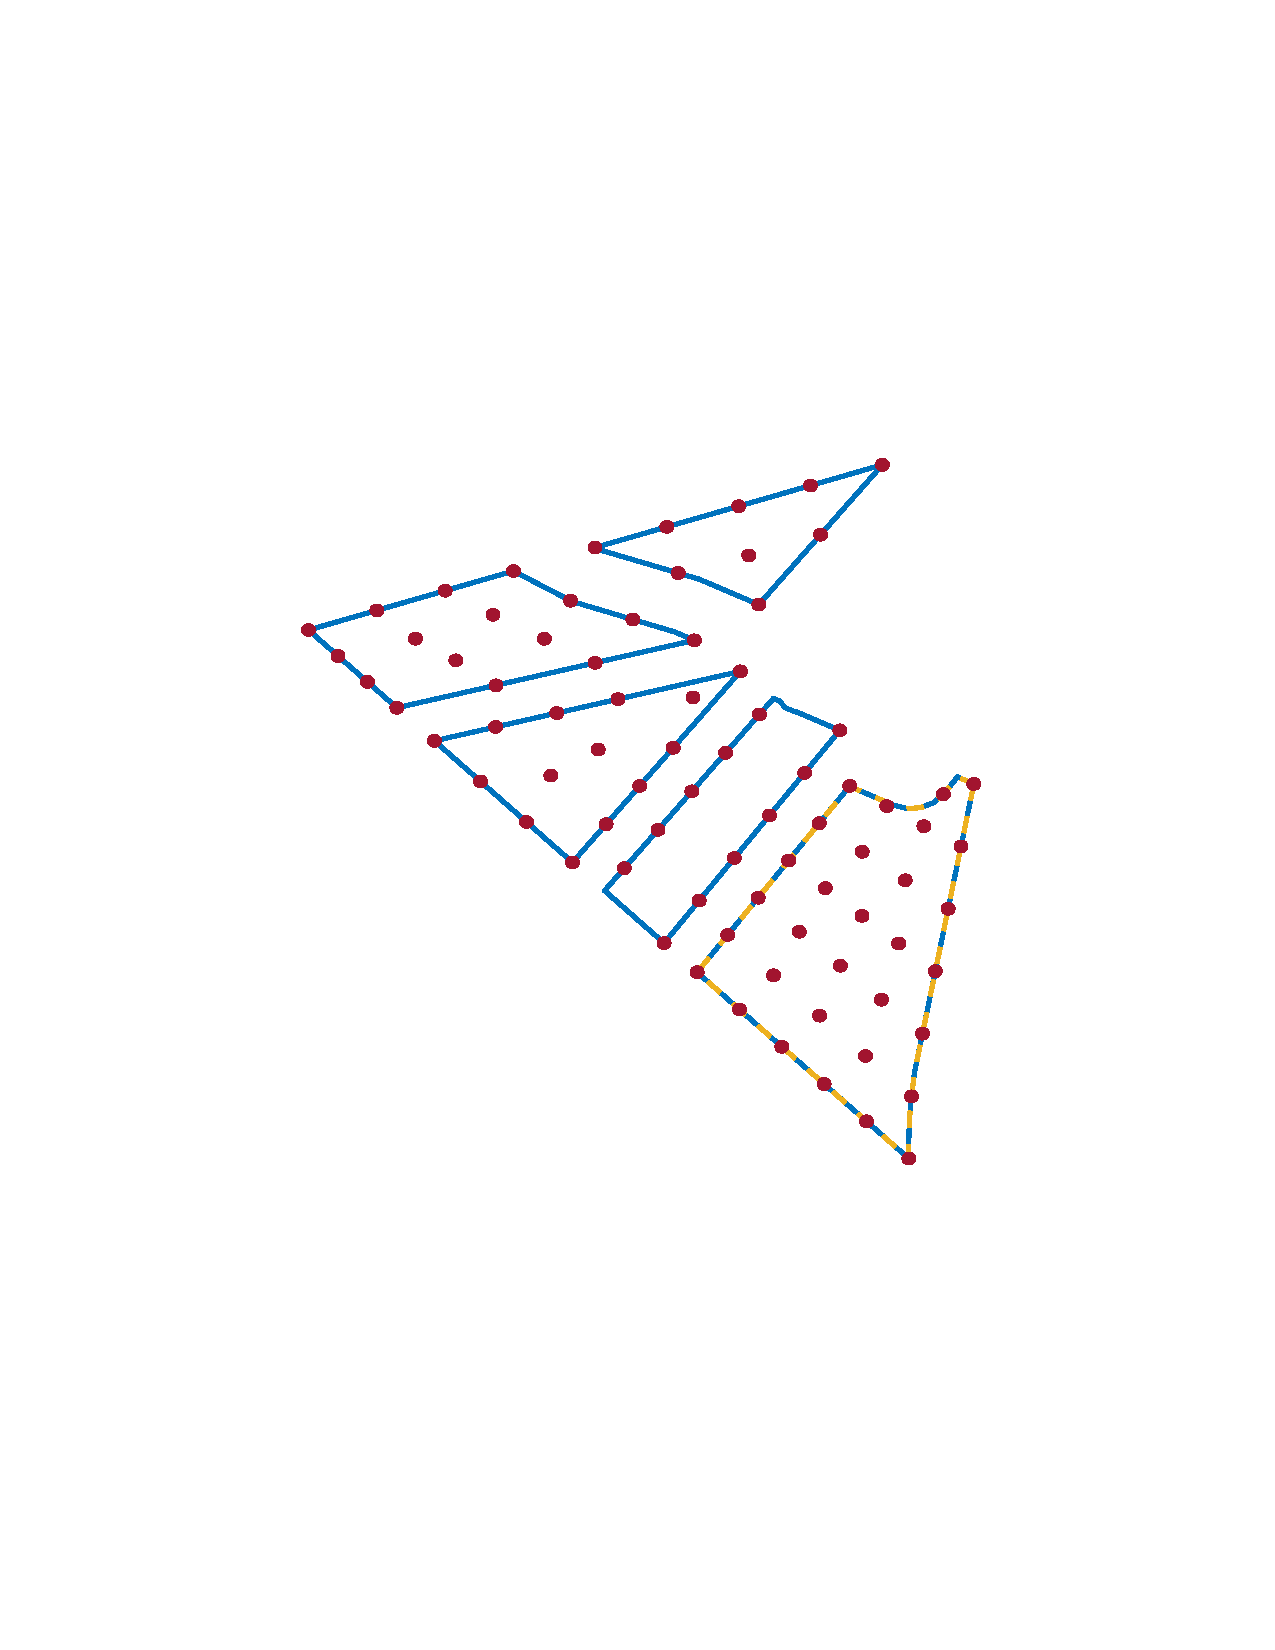
\includegraphics[width=3in, trim={2in 3.2in 1.8in 3.in},clip] {cs4Turbines.pdf}
            \caption{The wind farm boundary for cs3 (outlined in yellow) and cs4 (outlined in blue). A provided baseline turbine layout for cs4 is overlaid in red, with rotor radii to scale.}
            \label{fig:boundary}
            \end{center}
        \end{figure}


    \subsubsection*{Parameters}
    \label{sec:Parameters}
        The wind turbine is the IEA37 10 MW offshore reference turbine \cite{NREL10MW} with the following characteristics:
        \begin{center}
            \begin{tabular}{@{}lrl@{}}
            \toprule
                Rotor Diameter & 198 & m \\
                Hub Height & 119 & m \\
                Turbine Rating & 10 & MW \\ 
                Cut-In Wind Speed & 4 & m/s \\ 
                Rated Wind Speed & 11 & m/s \\ 
                Cut-Out Wind Speed & 25 & m/s \\
            \bottomrule
            \end{tabular}
        \end{center}

        \noindent All turbine data are also contained in the enclosed \texttt{iea37-10mw.yaml}. The power curve is defined as:   

        \begin{minipage}{0.53\textwidth}
            \begin{equation*}
                P(V) = 
                \begin{cases} 
                    0 & V < V_{\textit{cut-in}} \\
                    P_{\textit{rated}}\cdot\bigg(\frac{V-V_{\textit{cut-in}}}{V_{\textit{rated}}-V_{\textit{cut-in}}}\bigg)^3 & V_{\textit{cut-in}}\leq V < V_{\textit{rated}} \\
                    P_{\textit{rated}} & V_{\textit{rated}} \leq V < V_{\textit{cut-out}} \\
                    0 & V \geq V_{\textit{cut-out}}
                \end{cases}
            \label{eq:power}
            \end{equation*}
        \end{minipage}\quad
        \begin{minipage}{0.53\textwidth}
            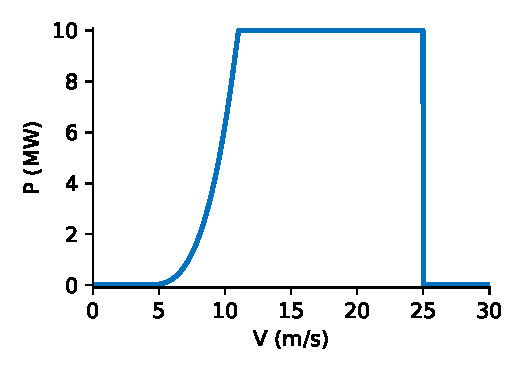
\includegraphics[width=2.6in]{power_curve.pdf}
        \end{minipage}

        For cs3 and cs4, the supplied wind resource is binned over both wind direction and wind speed.
        We supply a high number of frequency probabilities associated for each wind direction (60 values), and frequency probabilities associated with each wind speed's occurrence at each direction ($60\text{x}60=3600$ values).
        This is more data than needed for AEP convergence.  Participants are free to use any level of discretization or sampling strategy they prefer during the optimization (though final results will be compared using all 60 x 60 bins).  
        This data is included in \texttt{iea37-windrose-cs3.yaml}, which will be used for both cs3 and cs4.
        \Cref{fig:windrose} gives a graphical representation of the binned wind direction frequencies, and the wind speed sampling for a single wind direction.
       
        \begin{figure}[]
            \begin{center}
            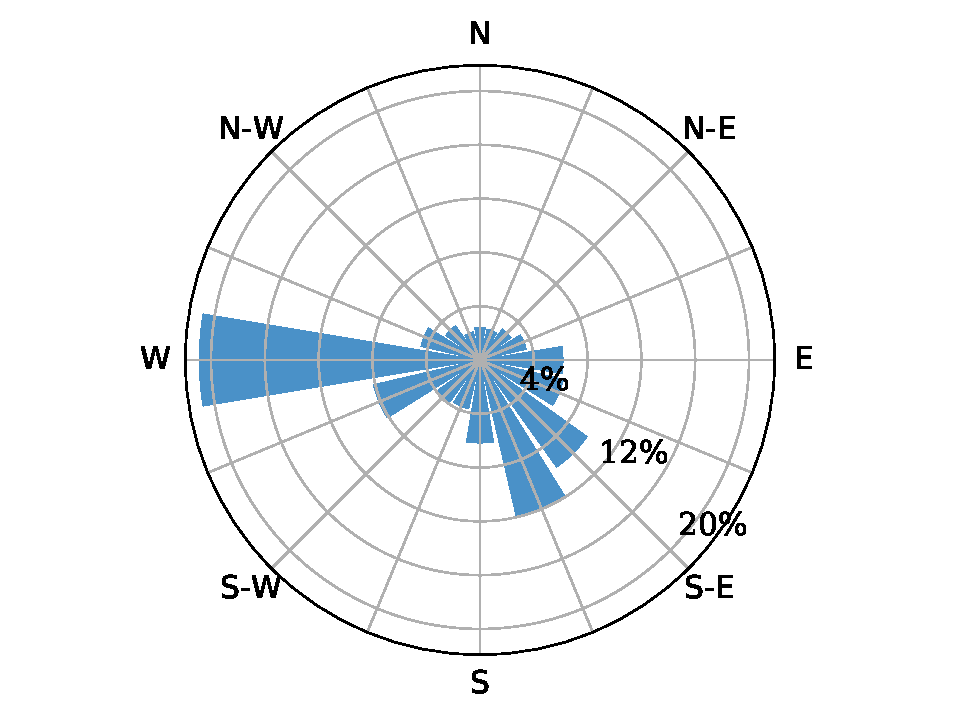
\includegraphics[width=3.25in, trim={.1in .8in 0.8in .8in},clip]{iea37-windrose.pdf}
            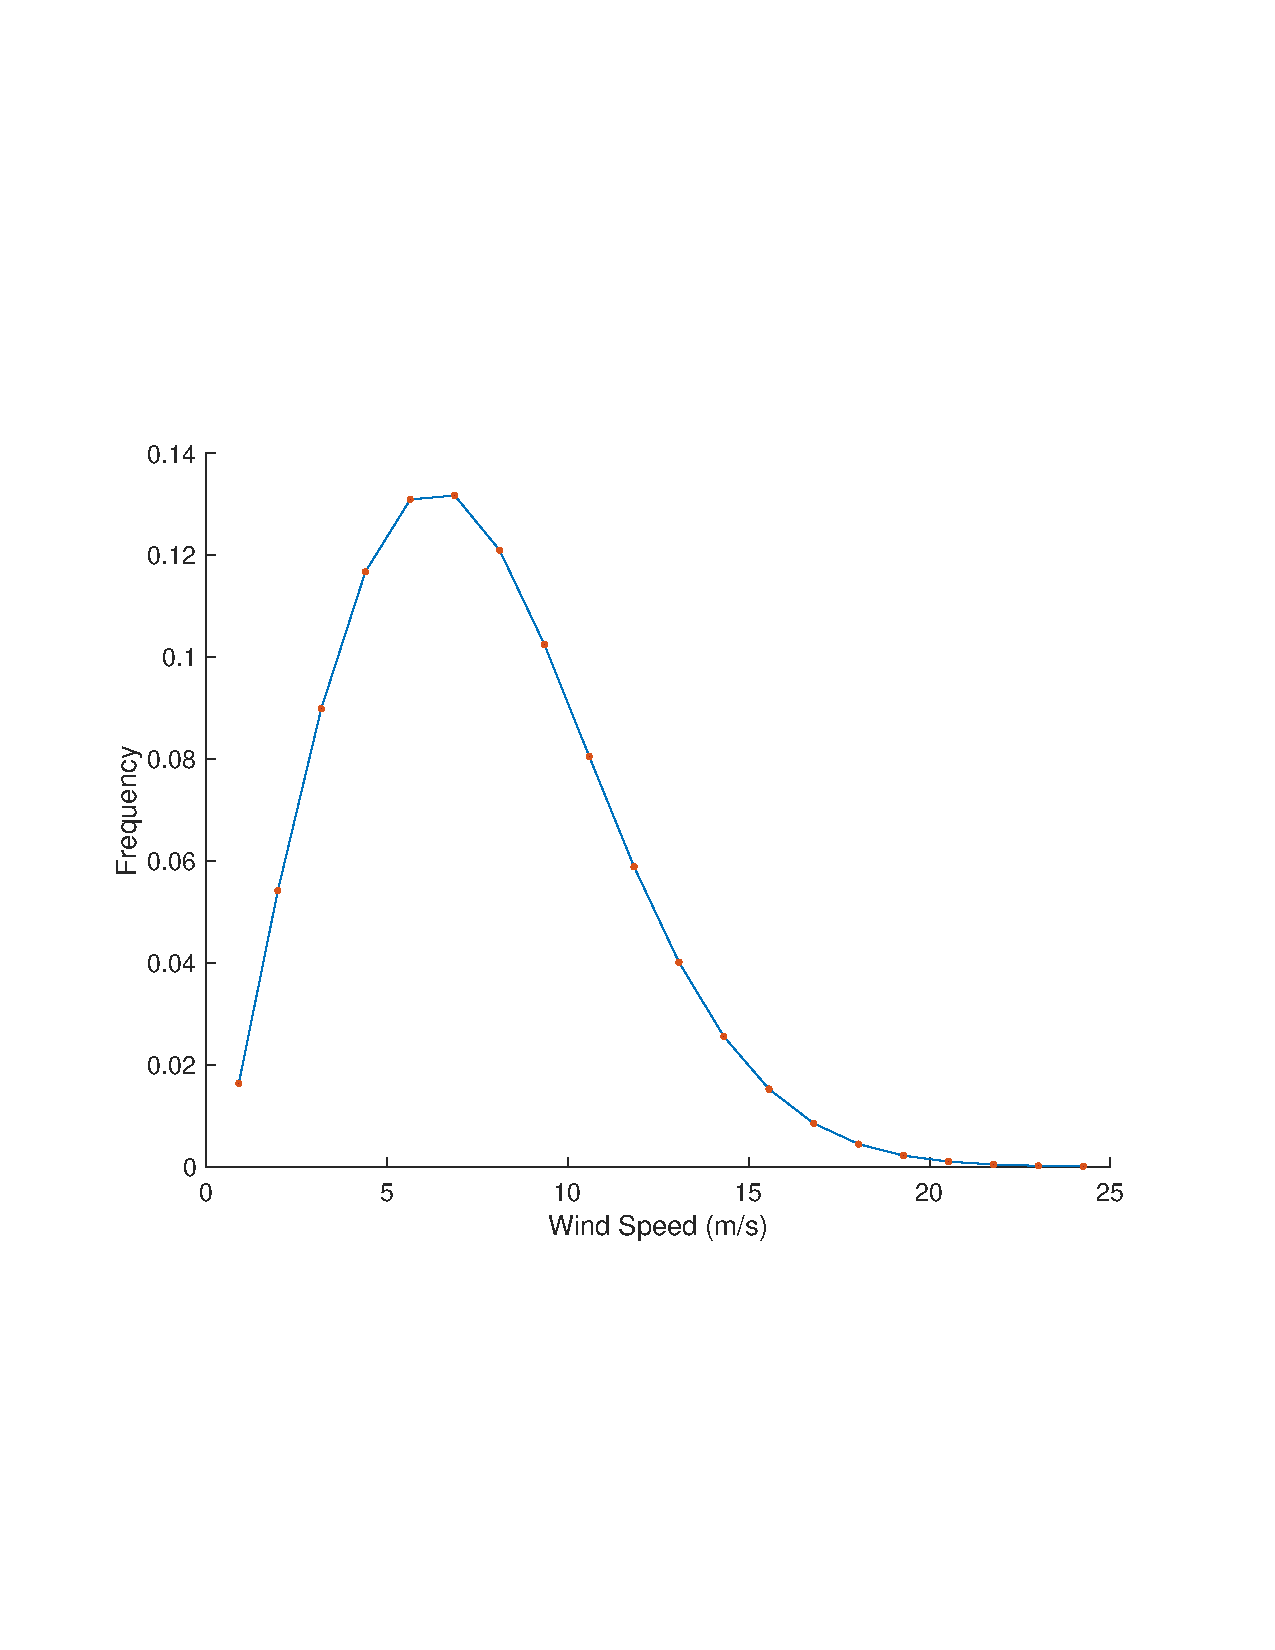
\includegraphics[width=3in, trim={.6in 2.72in 1in 2.4in},clip]{windspeed-freq.pdf}
            \captionof{figure}{(left) Wind frequency distribution over the 60 bins for the windrose used in cs3 and cs4. (right) Wind speed frequency distribution at one of the wind directions ($30^\circ$).}
            \label{fig:windrose}
            \end{center}
        \end{figure}


    \subsection{Case Study 3}

        This wind farm scenario consists of twenty-five (25) turbines with a boundary containing concavities.
        Participants will optimize the wind farm layout for maximum AEP with the provided Gaussian wake model, wind rose, turbine, and boundary.
        The wake model is supplied (coded in python) as \texttt{iea37-aepcalc.py}.
        Alterations to this implementation are permitted, as long as the governing physics equations are not altered.
        Participants may use other programming languages, but must use the same physics equations.
        To aid with this, the relevant equations are defined in a separate document (\texttt{iea37-wakemodel.pdf}), and baseline wind farm layouts with corresponding AEP values are provided in the \texttt{iea37-ex-opt\#.yaml} files to verify implementations.
    
    \subsection{Case Study 4}

        This scenario consists of eighty-one (81) turbines with a boundary containing concavities and discontinuities.
        The user is free to choose both the optimization algorithm and wake model.  This scenario contains discrete boundary regions.  The number of turbines in a given boundary region can be changed as long as the total number of turbines is fixed.  In other words, the participant or their optimization algorithm is free to move all eighty-one turbines between the five boundary regions.

\section{Reporting and Evaluation}

    \subsection{Baseline Layouts}
    \label{sec:BaselineLayouts}
        Baseline turbine layouts for both case studies are supplied.
        These are provided in part to give examples of our precise reporting format.
        They are called \texttt{iea37-ex-opt3.yaml}, \texttt{iea37-ex-opt4.yaml}, and \texttt{iea37-ex-log3.yaml}.
        Like the example layouts provided for case studies 1 and 2, these baseline layouts are also meant to provide a reasonable minimum output against which results can be measured.
        Participants are not required to use the baseline layouts as starting points for their optimizations, though they are permitted to do so.

    \subsection{Reporting}
    \label{sec:Reporting}
        Submissions must adhere to the \texttt{.yaml} format in order to enable easy and fast analysis of participant results.
        You will submit two (2) files per case study: one with your optimized turbine layout, the second a log of your optimization convergence data.
        Your submitted files should be named:
        
        \vspace{0.5em}
        \texttt{iea37-yourname-opt\#.yaml}
        
        \texttt{iea37-yourname-log\#.yaml}
        \vspace{0.5em}
        
        \noindent Where ``\texttt{yourname}'' is your personal or organizational name, all lowercase with no spaces or punctuation,
            \texttt{-opt\#.yaml} describes the ($x$,$y$) coordinates for your optimal turbine layout,
            \texttt{-log\#.yaml} contains information regarding your hardware and optimization algorithm's performance,
            and ``\texttt{\#}'' is the case study number of the submission (i.e. ``\texttt{-opt3.yaml}'' contains optimized results for cs3).

        %The following three files should be referenced internally by your submission, as is done by the baseline files:
        %\begin{itemize}
        %    \item \texttt{iea37-10mw.yaml} lists the turbine data for the used IEA37 10 MW offshore reference turbine.
        %    \item \texttt{iea37-windrose-cs3.yaml} describes the wind speeds and frequencies used in both case studies.
        %    \item \texttt{iea37-boundary-cs\#.yaml} gives the vertex outline of the wind farm boundaries.
        %\end{itemize}

        Of note, we require participants to log target function evaluations for \textbf{every} function call during the optimization process.
        As shown in the example log given in \texttt{iea37-ex-log3.yaml}, participants must report both: (1) number of total target function calls, and (2) AEP calculation at each chronological function call.
        To repeat, every call to the AEP calculation should be logged whether it is formally part of the optimization or not (e.g., each call in a finite difference estimate, each call in creating an initial population, etc.)
        % This means participants must log the intermittent AEP calculations at \textbf{each} function call occurring during the optimization process, in order for us to study trends regarding time to convergence.

    \subsection{Evaluation}
    \label{sec:Evaluation}
        Evaluations for cs3 will be made using the wake model target function supplied in \texttt{iea37-aepcalc.py} and convergence data reported by each participant.
        
        Because the participant wake models in cs4 are intended to differ, determining a ``best'' solution for cs4 is generally not possible.
        Evaluations will be made using a cross-comparison approach.
        Every participant will evaluate every other participant's solutions using their own wake model(s).
        It is essential that the \texttt{.yaml} format is adhered to so that cross-comparisons are painless.

\section{Participation}

    If interested (or potentially interested) in participating in either or both case studies send an email to \href{mailto:Nicholas.F.Baker@byu.edu}{the primary author} so we can keep you informed of updates/deadlines, etc.

\section{Enclosures}
    Files included with this document, needed for full participation in the case studies are:

    \begin{itemize}[noitemsep,topsep=0pt,parsep=0pt,partopsep=0pt]
        \item \texttt{iea37-10mw.yaml} - data for the reference turbine used in both cs3 and cs4
        \item \texttt{iea37-aepcalc.py} - target AEP calculator using a simplified Gaussian wake model
        \item \texttt{iea37-boundary-cs3.yaml} - the vertices for cs3's wind farm's boundary
        \item \texttt{iea37-boundary-cs4.yaml} - the vertices for cs4's wind farm's boundary
        \item \texttt{iea37-ex-log3.yaml} - example of optimization results, denoting timing and iteration analysis
        \item \texttt{iea37-ex-opt3.yaml} - baseline layout for cs3, template for your submitted optimal turbine layout
        \item \texttt{iea37-ex-opt4.yaml} - baseline layout for cs4
        \item \texttt{iea37-wakemodel.pdf} - description of the AEP algorithm used in cs3
        \item \texttt{iea37-windrose-cs3.yaml} - 60 bins, wind speeds given as Weibull distributions, for cs3 and cs4
    \end{itemize}

\bibliographystyle{aiaa}
\bibliography{iea37-wflocs-announcement}

\end{document}